\documentclass{article}

\usepackage{caption,color,fancyvrb,subfig}
\usepackage{code,algorithmic,algorithm}
\usepackage{graphicx,epsfig}
\usepackage{amsmath,amsthm,amsfonts}
\usepackage{amssymb}
\usepackage{setspace}
\usepackage{bibentry}
\usepackage[normalem]{ulem}

\nobibliography{prelim}

\textwidth = 6.5 in
\textheight = 9 in
\oddsidemargin = 0.0 in
\evensidemargin = 0.0 in
\topmargin = 0.0 in
\headheight = 0.0 in
\headsep = 0.0 in
\parskip = 0.12in
\parindent = 0.0in


\def\inv{^{-1}}

% \newcommand{\reminder}[1]{{\bf
%     [\marginpar[\hbox{{\Huge
%     $\bullet$}\raisebox{0ex}{\Huge $\longrightarrow$}}]%
% {\hbox{\raisebox{0ex}{\Huge $\longleftarrow$}{\Huge $\bullet$}}}#1]}}
% \newcommand{\pjk}[1]{{\bf
%     [\marginpar[\hbox{{\textcolor{blue}{pjk}}\raisebox{0ex}{\Huge $\rightarrow$}}]%
% {\hbox{\raisebox{0ex}{\Huge $\leftarrow$}{\textcolor{blue}{pjk}}}}\textcolor{blue}{#1}]}}
% \renewcommand{\pjk}[1]{\textcolor{blue}{[#1]}}
% \newcommand{\pete}[1]{\textcolor{red}{#1}}
% \newcommand{\change}[2]{\sout{#1} \textcolor{red}{#2}}


\begin{document}

\begin{titlepage}
\begin{center}

\textsc{\huge \bfseries \sc{Responsive Consistency in User-Centric}}\\
\textsc{\huge \bfseries \sc{Dynamic Network Environments}}\\[1.0cm]

\emph{A prospectus submitted in partial fulfillment of the degree of Doctor of
Philosophy}\\[5.5cm]

\textsc{\large DRAFT}\\
\emph{October 24, 2016}\\[2.0cm]

\emph{Preliminary Oral Examination for}\\
\textsc{\large Benjamin Bengfort}\\[2.0cm] % [4.0cm]
\emph{Advisor:} \\
\textsc{Dr. Peter J. Keleher}\\[.5cm]
\emph{Committee Members:}\\
\textsc{Dr. Bobby Bhattacharjee}\\
\textsc{Dr. Dave Levin}\\
\textsc{Dr. Neil Spring}\\[4.0cm]

{\bfseries Department of Computer Science}\\
{\bfseries University of Maryland, College Park, MD 20742}\\
{\bfseries December 9, 2016}
\vfill

\end{center}

\end{titlepage}

\newpage
\thispagestyle{empty}
\mbox{}


\newpage
\setcounter{page}{1}
\onehalfspacing
\begin{abstract}

Data replication has largely become the central technique in creating durable, highly available, multi-user systems and as a result the fault-tolerant coordination of replicas for correctness and consistency has become an increasingly important research area. As these systems have grown in scale and been deployed in geographically distributed clouds, the research focus has shifted away from networked file systems toward data-centric, cloud-managed database systems. One motivation for this shift has been the need to support an increasing number of mobile devices and another to provide scalability in collaborative workloads. However, with the advent of the Internet of Things and the increased use of multiple devices and local collaboration, we expect that local, user-centric clouds of heterogenous devices and mobile, dynamic networks will become increasingly important.

We contend that current consistency models are highly dependent on the network environment and that existing protocols can fail to achieve progress or provide sufficient consistency for user applications in many environments outside of the data center. Weak or eventual consistency models rely on the fast propagation of updates and therefore consistency is dependent entirely on message latency. Strong, sequential consistency provided by consensus protocols require multiple messages passed through a leader and though it can be shown that such protocols are correct, leadership introduces a bottleneck and partitions can lead to deadlock. In user-centric dynamic clouds, responsive consistency models must be developed to take advantage of the changing network environment and respond to user requirements.

We hypothesize that we can provide responsive consistency in heterogenous, mobile topologies through two mechanisms: the federation of multiple consistency models depending on the environment and the load balancing of leadership in a quorum through hierarchical consensus. Federated consistency allows heterogenous devices to select a variety of consistency polices that are integrated through a core consensus group. By allowing flexibility locally, devices can make progress through consistency models that take advantage of the current network environment, but still have global guarantees. Hierarchical consensus improves the core consensus group, making it highly available and scalable by balancing leadership to specific decision spaces based on access patterns. Together, we propose that Federated Consistency and Hierarchical Consensus provide a responsive consistency model that will enable an effective multi-user, distributed file system.

\end{abstract}
\setstretch{.5}

\newpage
\thispagestyle{empty}
\mbox{}

\newpage
\setcounter{tocdepth}{3}
\tableofcontents

\newpage
\listoffigures

\newpage
\onehalfspacing

\section{Introduction}

The rise of virtualized, on-demand computing resources and cloud computing has dramatically shifted the focus of research on consistency in distributed storage systems away from networked file systems toward geographically distributed database management systems, particularly key-value storage. These types of data systems benefit from low-latency, high-bandwidth connections where failure is common due to the magnitude of resources rather than inherent instability. As a result, ``eventually consistent'' (EC) \cite{vogels_eventually_2009} systems are said to be consistent enough for most workloads given some probabilistic bounding of staleness \cite{bailis_quantifying_2014,bermbach_eventual_2011,bailis_probabilistically_2012}. This has led consistency research towards investigating stronger forms of eventual consistency, primarily building upon Dynamo \cite{decandia_dynamo:_2007} and Cassandra \cite{lakshman_cassandra:_2010} as reference implementations. Alternatively, research into ensuring strong, sequential consistency (SC) or linearizability (LIN) in this environment has led to systems like Spanner \cite{corbett_spanner:_2013} which uses atomic and GPS clocks to ensure ``TrueTime'' for sequential ordering or a small number of master nodes that implement consensus algorithms \cite{lamport_paxos_2001,ongaro_search_2014} for locking or ordering \cite{kraska_mdcc:_2013}.

The focus on data center consistency has led to a centralized approach to data storage, forcing a modality where devices must connect to the cloud for file replication even when files exist in the local area \cite{drago_inside_2012}. Although this allows systems to ignore annoyances such as local network configuration and decentralized protocols it does present unnecessary overhead in terms of cost and latency. More pernicious, perhaps, is that users must now buy-in and store their data with a single provider that could go out of business or be hacked, which has lead to research in replicating local data with multiple untrusted cloud stores \cite{zhang_viewbox:_2014,feldman_sporc:_2010}. There are more devices than ever before connecting to storage applications, partially because users have multiple, heterogenous devices from wearables to workstations and partially because of the advent of the Internet of Things \cite{miorandi_internet_2012}. Cloud storage tends to be application specific, but with more devices and more users, \textit{generalized distributed storage} is required for collaboration and sharing that is not siloed and can be easily accessed by a variety of new platforms. Therefore we see a strong motivation to turn attention back to user-oriented networks of mobile heterogenous devices that do not have the benefit of data center level connectivity.

We propose to explore consistency mechanisms in \textit{user-centric dynamic clouds}: a multi-user tapestry of mobile, heterogenous devices connected via variable-latency and partition-prone networks that change over time. These types of clouds are interesting and we believe that the unique challenges of this network environment require specialized consistency models in order to be effective. Because of the user-centric nature of this research, the requirement for collaboration and sharing, and in order to generalize distributed storage in this type of cloud we further propose the study of a file system as the primary data storage application. File systems must be highly available such that a user does not notice any delay due to coordination but must also have strong consistency such that any conflicts are presented to the user as soon as possible. These two requirements together provide a challenge for any single consistency model, particularly when the devices in the file system are mobile, can be turned off, and may have a variety of resource constraints.

Our core contention is that \emph{consistency depends on the
``environment''}. In a file system, the two primary symptoms of inconsistencies are version forks and stale reads. ``Weak'' (EC) systems depend on disseminating new writes quickly in order to prevent forks and stale reads. A ``strong'' (Raft consensus) system without caching might be provably correct, but might fail to make progress as network conditions deteriorate. Furthermore, file caching is essential to providing usable performance for any file system. Caching (without expensive validations) leads to stale reads. Forks can happen even without caching unless locking is used, however locks are too expensive for data center environments, much less user-centric dynamic clouds. Hence, a strong (Raft) system does not necessarily provide strong consistency guarantees on individual application-level file accesses. Further, the extent to which the system diverges from SC increases with decreasing network quality.

In order to provide any consistency guarantees in a dynamic environment the consistency model must be \textit{responsive}, providing flexibility when the network is unavailable or laggy and providing strong consistency guarantees when stable connections exist. Our approach focuses on two primary techniques to provide responsiveness: the \textit{federation} of weak but available consistency mechanisms with sequential consistency by consensus and the use of \textit{hierarchical} consensus to scale consensus groups beyond a handful of devices. ``Federated Consistency'' allows devices to switch local consistency models depending on the use case or to adapt consistency protocols automatically as the network environment changes, optimizing for strong consistency or availability as required. ``Hierarchical Consensus'' increases the availability of a consensus group by creating decision localities of interest based on accesses to particular objects by a particular group of devices. Both models are flexible locally, but can provide global system guarantees, guarantees we propose to explore in this research.

We hypothesize that the integration of multi-modal consistency with hierarchical centralized leadership via consensus will lead to higher availability than strong consistency models but provide stronger guarantees than eventually consistent systems. We will quantitatively demonstrate the efficacy of such a system through simulation and by implementing a file system, FlowFS, and testing it under real-life workloads. By comparing FlowFS to homogenous systems with similar sizes and topologies and measuring the number of inconsistencies and amount of latency in both simulation and a real world implementation we will show that responsive, flexible consistency protocols are more available and provide stronger guarantees than their homogenous counterparts in user-centric dynamic personal cloud topologies.

The rest of the proposal is organized as follows: first, we will present background and related work on consistency models, consensus protocols, and replication. We will then describe our preliminary work: network simulations of a variety of consistency protocols and an exploration of the effect of environment on consistency. We will then proceed to describe Federated Consistency in detail, work that we have also already investigated in simulation. Next, we will present our initial thoughts on Hierarchical Consensus and extensions on both federation and hierarchical consensus to improve performance such as automatic adaptation. We conclude with a proposed timeline and set of research goals towards a dissertation.

\section{Background and Related Work}

Our work is primarily grounded in data-centric consistency models. These models previously thought of as discrete levels, e.g. weak and strong, have more recently been viewed as a continuum \cite{yu_design_2002,afek_quasi-linearizability:_2010}. To provide background to consistency mechanisms in dynamic environments, we will start by defining a generalized log-based consistency model then extend it to our more file-system specific, primary metric: \textit{forks}. We will then explore various consistency levels on the consistency continuum: weak, eventual, causal, sequential, and linearizable expressed both in terms of the generalized model as well as how they perform in a file system context. This grounding primarily provides background to our first responsive approach: Federated Consistency.

Federated Consistency is a form of hybrid consistency where several consistency protocols are integrated in a single system. Because our preliminary work has focused on federation, we will present a detailed review of related work on hybridization and consistency rationing. We hypothesize that by integrating both eventual and sequential consistency such that there is a strong central core, similar to the architecture presented by Oceanstore \cite{kubiatowicz_oceanstore:_2000}, Federated Consistency will be able to provide stronger guarantees and centralized conflict resolution than other weaker consistency models, while providing flexibility and availability in variable latency environments.

The strong central core must provide at least sequential consistency, a consistency level that is generally coordinated via a consensus protocol. Therefore, in the second part of the background, we will present consensus protocols, starting by a review of Paxos \cite{lamport_paxos_2001} and its various flavors. We have selected Raft \cite{ongaro_search_2014} as our consensus protocol of choice, and therefore describe its operation in particular detail. Our review of consensus is intended to present the motivation and discussion of Hierarchical Consensus -- an extension of Raft that load balances the leader across decision spaces (groups of related objects) based on access patterns. Finally, in the last section of the background, we will review topics in replication that are critical to our work and present related systems already implemented.

\subsection{Consistency}

Our consistency model is a \textit{data-centric} model, as opposed to a \textit{client-centric} model, which has been generalized in recent literature by two primary facets: ordering and staleness \cite{bermbach_consistency_2013}. Client-centric models view the system as a black box and consistency is described as guarantees made to processes or applications interacting with the system such as ``read your writes'' or ``write follows read'' \cite{vogels_eventually_2009}. Data-centric consistency on the other hand is concerned about the ordering of operations applied to a replica and generally considers the problem of how those operations relate to each other in a per-replica, append-only log. This generalization is different than a file-system specific view of consistency, but gives a method for comparing different consistency protocols along increasing strictness of ordering and staleness.

We can generalize data-centric consistency as follows: each replica is a state machine that applies commands in response to client requests or messages from other replicas. Each command is appended to a log that records the time ordered sequence of commands such that an entry at the end of the log happened before the previous entry. Replicas are locally consistent if they are in a similar state expressed by the relative condition of their logs (note that this generalization will translate well to a discussion of consensus in the next section); they are globally consistent if they are in a similar state to some abstract global ordering that meets one or more criteria. In either case, consistency guarantees can be described along two dimensions: staleness and ordering as follows:

\begin{enumerate}
    \item \textit{Staleness} refers to how far behind the latest global state a local log is and can be either expressed by the visibility latency of distributing a command to all replicas or simply by how many updates the log is behind by.
    \item \textit{Ordering} refers to how closely individual logs adhere to an abstract chronological ordering of commands. A strict ordering requires all logs or some prefix of the log to be identical, whereas weaker ordering allows some divergence in the order updates are applied to the log.
\end{enumerate}

Most data-centric consistency models do not consider staleness but instead refer to the strictness of ordering guarantees and the method by which updates are applied to the state of the replica \cite{tanenbaum_distributed_2007}. This is primarily because enforcing ordering strictness leads to increased staleness. This occurs in two ways: increased coordination introduces delays between the issuance of a command and its local application and through dependencies that require dependent commands to be applied before the command in question. While staleness is easy to quantify in terms of time (t-visibility) and versions (k-staleness) \cite{bailis_quantifying_2014}, ordering is very difficult to quantify. Therefore in order to generalize to consistency models beyond eventual consistency, our model considers the specific symptoms of ordering inconsistency in a file system context: \textit{forks} and \textit{stale reads}.

\subsubsection{File System Consistency}

We define a file system as a hierarchical namespace of object \textit{versions} where a version represents the immutable state of a particular object at a specific time \cite{helland_immutability_2015}. The \textit{view} of a file system is the set of locally cached versions, usually the latest version, for each object. Accesses to specific objects, e.g. read and write, update the local view of the file system and must be replicated in order for the file system to be consistent across replicas.

We propose a file-system specific consistency model that extends the generalized log ordering consistency method. In this model, commands are file accesses to a single object and each replica maintains a single, ordered log of accesses. Write accesses update the state of the file system (or view) by creating new versions of objects; read accesses update the state by determining the most recent version of the object either via the local cache or via a remote access. A \textit{stale read} is defined as a read to the local cache that returns a version of the object that is behind the latest global version. The ordering of reads and writes in the log determines the chronological sequence of all accesses to the file system and therefore defines the version history.

Each \textit{version} is a piece of meta data that describes an object state at a particular time and is identified by a monotonically increasing, conflict-free version number \cite{parker_detection_1983}. Versions can contain dependency information, and in particular one dependency is required for all versions: the version of the parent upon whose access created the resulting version. An object's version history is therefore a tree, though the desired history is a single sequence or chain of unbroken updates to the object. Inconsistency in a file system is therefore a divergence in the linear history of the set of objects in the namespace and can be measured in terms of \textit{forks}.

\begin{figure}
    \centering
        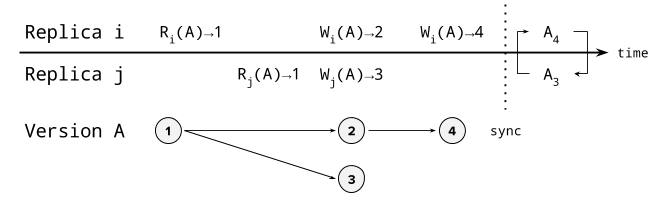
\includegraphics[width=.9\textwidth]{figures/forks}
        \caption{Forks branch sequentially ordered version numbers}
        \label{fig:forks}
\end{figure}

\begin{description}
    \item[\textbf{Fork}] A fork occurs when two replicas concurrently write a new version to the same parent object as shown in Figure \ref{fig:forks}. Forks introduce inconsistency because there are now two potential orderings of updates to the log, but forks are primarily the symptom of staleness; e.g. the second writer wrote to a stale version of the object.
\end{description}

There are two primary causes of forks: concurrent accesses by multiple replicas (a true conflict between multiple writers) and stale reads. The former is distinguished from the latter only if the possibility of synchronization (a process to bring replica logs to the same state) could have occurred. From the point of view of the system, they are identical causes. Forks can branch to arbitrary lengths as replicas continue to write to their latest local copies, however when synchronization occurs a decision as to which ordering of writes is correct must occur. Note that conflict in this consistency model refers to the concurrent access of the same or dependent objects. In fact, it is possible that the concurrent access to two independent objects causes two different, valid orderings -- however because it is difficult to implicitly define objects that are independent from each other, consistency definitions do not take this conflict into account.

\subsubsection{Discrete Consistency Levels}

In this section we will identify several discrete consistency levels in order of increasing strictness of the ordering of their logs as defined by the generalized log consistency model presented by Bermbach and Kuhlenkamp \cite{bermbach_consistency_2013}. The relationship between these consistency models indicates that there is a continuum of consistency based on the strictness of ordering. We will also note, where possible, the effect of the consistency model in terms of file-system specific consistency and forks.

\textit{Weak consistency (WC)} is is the least strict consistency model.
A weakly consistent system makes no guarantees whatsoever about the relationship of local to remote writes and whether or not any given update will become visible \cite{vogels_eventually_2009}. Weak consistency is often described as ``replicas might get lucky and become consistent'' and in fact a weakly consistent implementation may not have a synchronization protocol whatsoever \cite{bermbach_consistency_2013}. For this reason, we do not consider weak consistency in general except to identify it as a baseline.

\textit{Eventual consistency (EC)} is primarily concerned with the final state of all logs in the system given some period of quiescence that allows the system to converge. In this case, all replicas, no matter their log ordering, should have identical final versions for all objects in the namespace. This suggests that eventual consistency requires some \textit{anti-entropy} mechanism to propagate writes and a policy to handle convergence \cite{terry_managing_1995}. Eventual consistency is very popular for NoSQL databases and hosted distributed storage services \cite{decandia_dynamo:_2007,lakshman_cassandra:_2010} because it allows an optimistic approach to consistency: conflicts are rare in most systems, if something does go wrong, conflict resolution is passed to the application layer. In practice, most applications can handle some inconsistency and moreover the small inconsistency windows due to low latencies in cloud data centers make such conflicts rare and short-lived enough to be worth the risk \cite{bailis_quantifying_2014}.

Eventual consistency implemented by a \textit{last writer wins} policy simply accepts all writes so long as they are more recent than the latest local versions. Eventual reads and writes are always performed on local caches and are therefore highly available since they return a response to accesses immediately. Eventual consistency does allow forks to occur and moreover allows individual replica logs to have wholly different orderings so long as the last version for each object is in the same given no accesses have occurred for a long enough period of time. As a result, the latest version of an object may alternate between writes to competing forks (a fairly weak semantic) and in this case, it is up to the application to detect the inconsistency. However, EC logs do have one important property - for each object, every write in the log is ordered in a monotonically increasing fashion.

\textit{Causal Consistency (CC)} ensures that all writes which have causal relationships have those dependencies satisfied (inserted into the log) before the write can become visible \cite{ahamad_causal_1990}. Therefore, even though a write might have been propagated to another replica server it cannot be read until all of its dependencies have also been propagated. Causal consistency can increase staleness particularly when implicit or potential causality creates large dependency graphs that must be resolved before writes can be applied \cite{lloyd_dont_2011}. This can be managed by allowing the application to explicitly specify the dependencies for each write \cite{bailis_potential_2012}. Causal consistency is often referred to as the ``strongest form of consistency for highly available systems'', however CC does not require replica convergence \cite{guerraoui_consistency_2002} though with a few modifications including a convergence mechanism, it can easily be bolted on to an eventual system \cite{bailis_bolt-causal_2013}.

Eventual and causal consistency are both weak forms of consistency that are designed for high availability; that is they can respond to requests immediately from a local cache without coordination. Conflict detection and resolution are therefore critical processes asynchronous with the accesses that cause the conflict. These types of consistency are well suited for network environments that are partitioned or such that effective coordination is not available at the time of the access; e.g. for a user working on an airplane with no connectivity. The following strong consistency models, on the other hand, require coordination at the time of the access, detecting and eliminating conflict synchronously.

\textit{Sequential consistency (SC)} is a strong consistency model that requires that all replicas have the exact same ordering of their logs, such that all writes by all clients are appended in the same exact order \cite{attiya_sequential_1994}. Sequential consistency is not strict in that it does not make guarantees about staleness (or the ordering of reads) but does require that all writes become visible in the same order \cite{bermbach_consistency_2013}. Sequentially consistency is typically implemented with consensus algorithms such as Paxos \cite{lamport_fast_2006} or Raft \cite{ongaro_search_2014} that coordinate logs by defining a transitive, global ordering for all conflicts. Alternatively, sequential consistency and can be implemented with warranties -- time based assertions about a group of objects that must be met on all replicas before the assertions expired \cite{liu_warranties_2014}.

\textit{Linearizability (LIN)} is the strongest form of consistency; not only must all write operations occur in sequence, but all operations including reads must be ordered chronologically \cite{herlihy_linearizability:_1990}. A consensus algorithm alone cannot implement linearizability and instead some distributed locking mechanism is required. For example a consensus algorithm can be adapted to instead of making decisions about the total ordering of conflicting writes, granting or releasing locks from requestors, however this opens up the potential for deadlock and extremely poor performance, defeating the purposes of replication in the first place! Data center environments that don't have to deal with issues of clock skew by using super precise atomic and GPS clocks can use precise time measurements to enable a distributed two phase commit protocol \cite{corbett_spanner:_2013}, however every replica is required to have such a time piece, which is not practical for heterogenous topologies.

\subsubsection{Consistency Rationing and Hybridization}

Federated Consistency attempts to integrate multiple consistency levels as described in the previous section into a hybrid consistency model such that there is a separation between the local availability and consistency trade-off and global consistency guarantees. For example, the hybridization of an eventual consistency cloud of devices with a strong sequential core allows eventual nodes to make progress, while minimizing the effect of convergence delay on consistency. In this section, we will review work related to this style hybridization.

One of the earliest attempts to hybridize weak and strong consistency was a model for parallel programming on shared memory systems by Agrawal et al \cite{agrawal_mixed_1994}. This model allowed programmers to relax strong consistency in certain contexts with causal memory or pipelined random access in order to improve parallel performance of applications. Per-operation consistency was extended to distributed storage by the RedBlue consistency model of Li et al \cite{li_making_2012}. Here, replication operations are broken down into small, commutative suboperations that are classified as red (must be executed in the same order on all replicas) or blue (execution order can vary from site to site), so long as the dependencies of each suboperation are maintained. The consistency model is therefore global, specified by the red/blue ordering and can be adapted by redefining the ratio of red to blue operations, e.g. all blue operations is an eventually consistent system and all red is sequential.

The next level above per-operation consistency hybridization is called \textit{consistency rationing} wherein individual objects or groups of objects have different consistency levels applied to them to create a global quality of service guarantee. Kraska et al. \cite{kraska_consistency_2009} initially proposed consistency rationing be on a per-transaction basis by classifying objects in three tiers: eventual, adaptable, and linearizable. Objects in the first and last groups were automatically assigned transaction semantics that maintained that level of consistency; however objects assigned the adaptable categorization had their consistency policies switched at runtime based on a cost function that either minimized time or write costs depending on user preference. This allowed consistency in the adaptable tier to be flexible and responsive to usage.

Chihoub et al. extended the idea of consistency rationing and proposed limiting the number of stale reads or the automatic minimization of some consistency cost metric by using reporting and consistency levels already established in existing databases \cite{chihoub_harmony:_2012,chihoub_consistency_2013}. Here multiple consistency levels are being utilized, but only one consistency model is employed at any given time for all objects, relaxing or strengthening depending on observed costs. By utilizing all possible consistency semantics in the database, this model allows a greater spectrum of consistency guarantees that adapt at runtime.

Al-Ekram and Holt \cite{al-ekram_multi-consistency_2010} propose a middleware based scheme to allow multiple consistency models in a single distributed storage system. They identify a similar range of consistency models, but use a middleware layer to forward client requests to an available replica that maintains consistency at the lowest required criteria by the client. However, although their work can be extended to deploying several consistency models in one system, they still expect a homogenous consistency model that can be swapped out on demand as client requirements change. Additionally their view of the ordering of updates of a system is from one versioned state to another and they apply their consistency reasoning to the divergence of a local replica's state version and the global version. Similar to SUNDR, proposed by Li et al. \cite{li_secure_2004}, an inconsistency is a fork in the global ordering of reads and writes (a ``history fork''). Our consistency model instead considers object forks, a more granular level that allows concurrent access to different objects without conflict while still ensuring that no history forks can happen.

\subsection{Consensus}

Consensus algorithms are generalized as replicated state machines where a quorum of replicas must coordinate to decide on the application of a command that will change the local state of the replica \cite{schneider_implementing_1990}. By keeping a log of all applied commands, consensus is fault-tolerant because an offline node that rejoins the quorum can replay the commands to return to the same state as the other replicas.   Moreover, so long as a majority of nodes are online, the quorum can be said to be available, in that it will respond to requests that access the state. Because accesses can be seen as commands modifying the visible state of the object namespace, and because the command log is identical to the consistency logs described in the last section, we can say that consensus algorithms can be used to provide strong consistency at the cost of multiple coordination messages per access.

Most consensus algorithms in the literature are variations of the Paxos algorithm \cite{lamport_paxos_2001}, and more specifically the Fast Paxos implementation \cite{lamport_fast_2006}. Paxos proposes three phases to safely apply a command to the state machine: \textit{prepare}, \textit{propose}, and \textit{accept}. All phases are two stages, the first a vote and the second a broadcast of the results of the vote. In the prepare phase, a replica attempts to establish the master replica for a specific command by broadcasting a ballot number and getting majority agreement that the ballot (the entry at the log at that position) is owned by the master. The second phase broadcasts the value and receives a majority vote if that state can be successfully applied. The third phase accepts (commits) the result to the state machine. The primary variation, Fast Paxos, bundles multiple requests by reserving ballot numbers ahead of time to eliminate the \textit{prepare} phase (which is why most descriptions of Paxos generally identify only two phases). One way we can think of this is as the election of a primary leader in the quorum.

Because of the multiple round-trips necessary to achieve consensus, many variations of Paxos have been proposed to improve performance. For example S-Paxos \cite{biely_s-paxos:_2012} attempts to distribute the workload of the leader, Multi-Paxos \cite{camargos_multicoordinated_2007} allows multiple leaders per round, Flexible Paxos \cite{2016arXiv160806696H} allows for multiple quorum intersections, and Egalitarian Paxos \cite{moraru_egalitarian_2012,moraru_there_2013} allow fast and slow track voting. These variations tend to be optimistic in that conflict occurs rarely and that it can be detected by the consensus algorithm, allowing for repair if necessary.

\subsubsection{Raft}

Paxos has been shown to be very difficult to correctly implement and verify \cite{chandra_paxos_2007} and although attempts have been made to highlight the practicality of a subset of the Paxos guarantees \cite{mazieres_paxos_2007} it has been shown that Paxos is not easily understandable. To that end, we have used the Raft consensus protocol \cite{ongaro_search_2014,howard_raft_2015} as our primary consensus implementation in our preliminary investigations. The protocol is described briefly as follows.

Every Raft node can be in one of three states: \textit{follower}, \textit{candidate}, and \textit{leader} and are initialized in the follower state. The system has two primary timing parameters: the election timeout and the heartbeat interval. When in follower and candidate mode, a timeout is randomly selected from the election timeout range, and if the timeout occurs the node will become a candidate and start an election to become leader. If a majority of nodes vote yes to that candidate then the node switches to the leader state and begins sending \texttt{AppendEntries} messages at the rate of one at least every heartbeat interval. If a follower or a candidate receives a valid \texttt{AppendEntries} message, it resets its election timeout by selecting a new random timeout from the election timeout range. The relationship between the heartbeat interval and the election timeout must be such that at least two heartbeats can arrive before the node switches to candidacy. The random selection of a timeout prevents thrashing if all nodes are started at the same time.

Once elected leader, all accesses are forwarded to that node. Leaders maintain a term identification, a monotonically increasing global number. If a message comes in with a remote term higher than the local, then that node must switch to being a follower and update their local term. Accesses and their terms are sent to all followers in \texttt{AppendEntries} messages. Followers compare their terms to the access term, and if a majority of followers accept the access, then the leader sends a commit message in the following \texttt{AppendEntries} RPC message.

% \subsubsection{Consensus Trees}
% NOTE: Wanted to put in related works, similar to consistency discussion.

\subsection{Replication}

Consistency and consensus are generally separate issues from the actual replication of both metadata and data in a distributed storage system. In fact, consistency only requires the replication of \emph{metadata} because it is the metadata that defines the view or state of the system \cite{chandy_distributed_1985}. In fact, given that data can be replicated as immutable chunks or blocks identified by a hash function, the problem of replicating data is one of service availability \cite{venkataramani_operating_2002} or data locality \cite{kuenning_automated_1997} not one of locality. Therefore for the purposes of this research, we focus on the consistent replication of metadata.

We have explored two primary methods of replication in a distributed file system: gossip and broadcast protocols. As a rule, limiting the number of messages sent during replication is important as the number of messages is a good metric for resource usage and constraints such as available bandwidth or message processing capability. Gossip protocols are generally used as anti-entropy to disseminate information across the network in an epidemic fashion. Because gossip protocols use peer-to-peer connections, there are only as many messages per gossip interval as there are pairwise associations. Broadcast replication, on the other hand, can quickly overwhelm a system if all nodes are broadcasting a message to all other nodes, but is used well in centralized systems such as the Raft protocol where only a leader broadcasts and followers respond to the leader.

Gossip protocols (often called rumor spreading) are a form of epidemic information spreading that do not require central coordination \cite{kempe_gossip-based_2003, karp_randomized_2000}. On a routine interval, specified by the \texttt{anti-entropy delay} timing parameter, a replica will randomly select one of the other replicas in the system and exchange information. Because all nodes are randomly selecting another node at every interval, information travels quickly through the network in an exponential fashion and provide high fault-tolerance and even automatic stabilization. Generally speaking there are two types of gossip: \textit{push} and \textit{pull}. Push methods simply forward all locally updated information to the remote node on the anti-entropy interval. Pull methods require two phases: a request for information after a certain period and the response from the remote node.

Several replication protocols have directly influenced or inspired our work. Bayou \cite{terry_managing_1995,terry_session_1994} is an eventually consistent system that implements anti-entropy as its replication mechanism and conflict resolution by some primary or trusted centralized server. SUNDR \cite{li_secure_2004} is a secure file system that integrates local and cloud storage and detects inconsistencies by identifying forks, our primary inconsistency metric. The Ori File System \cite{mashtizadeh_replication_2013} replicates file history and allows the merge and grafting of histories similar to Git trees. As a result branches and forks are also a big part of the Ori methodology as are complex data structures for grafting and dealing with conflict. Finally, the Stellar consensus protocol \cite{mazieres_stellar_2015} provides federated byzantine agreement through the use of quorum slices.

\section{Preliminary Work}

We have begun our investigation into the relationship between network environment and consistency by building a discrete event simulator in Python using SimPy that allows us to easily characterize networks and consistency protocols. Furthermore we have utilized the simulator to investigate \textit{Federated Consistency} and have made progress by obtaining experimental results. In this section, we will describe the simulator and the investigation that led to the core proposal of Federated Consistency and Hierarchical Consensus. In the proposed work section, we will explore Federated Consistency in greater detail.

The simulator has two primary components: workload generators and device processes. Workload generators act as clients (users) that issue read and write accesses to named objects and are generally associated with a single device process such that the access is associated with a local replica. Device processes represent, for the most part, replica servers that are connected to each other through a specific topology. Devices respond to accesses, generate replication messages, and respond to messages from other devices. The input to a simulator therefore is a topology that defines the devices, their specific properties, and connections as well as an workload trace or set of parameters to generate random, realistic workloads. Experiments are conducted by running multiple simulations in parallel with different combinations of the above parameters.

Because most research on gossip protocols and consensus algorithms specify small topologies of a size that provide a minimum level of fault tolerance, our first question related to the scalability of consistency protocols to topologies with increasing numbers of nodes. To answer the question, we designed an experiment with 30 independent simulations: 15 differently sized topologies from 5 to 145 devices and two homogenous consistency protocols. This example serves to demonstrate the methodology behind our simulations as well as highlight a number of the tunable knobs that allow us to explore our proposal in greater detail.

The simulations implemented either eventual consistency via bilateral gossip and a latest-writer wins policy or sequential consistency via Raft consensus. The simulation specified the topology as a variable number of devices in five locations, such that devices in a single location benefited from local area network latency and connections between locations were considered wide area.  Local area latencies were normally distributed with mean latency, $\lambda_{\mu}=30$ms and standard deviation of latency, $\lambda_{\sigma}=5$ms; whereas wide area latencies were higher and more variable, $\lambda_{\mu}=300$ms and $\lambda_{\sigma}=50$ms. The workload was specified as a static

Both EC and SC implementations rely on timing parameters for the gossip interval as well as Raft timeouts. In order to define a relationship between consistency models, these timing parameters are defined by network latency. We first computed a conservative timing parameter given as $T=10\lambda_{\mu}$ based on the wide area latency mean. The anti-entropy interval for Eventual consistency is given as $\frac {T} {4} = 750$ms. For Raft, the heartbeat interval is $\frac {T} {2} = 1500$ms and the election timeout is a uniform random selection in the range $U(T, 2T) = U(3000, 6000)$. These conservative timing parameters ensure that it is rare that messages arrive out of order, even in highly variable connections.

The simulation workload was defined as a static trace of accesses such that all simulations received the same exact accesses. Each device implemented a workload of read and write accesses on a local namespace of 15 objects. Conflicts were introduced to the simulation by overlapping a subset of the local namespace of each device with the other device namespaces, specified by a probability of conflict, $P_c$. In this simulation, $P_c=0.3$ meaning that 30\% of the objects accessed on each device would also be accessed on another device. Accesses were issued at intervals normally distributed with the access interval mean, $A_{\mu}=3000$ms and the access interval standard deviation, $A_{\sigma}=380$ms such that accesses were roughly related to the timing parameter.

\begin{figure*}
    \centering
    \minipage{0.48\textwidth}
      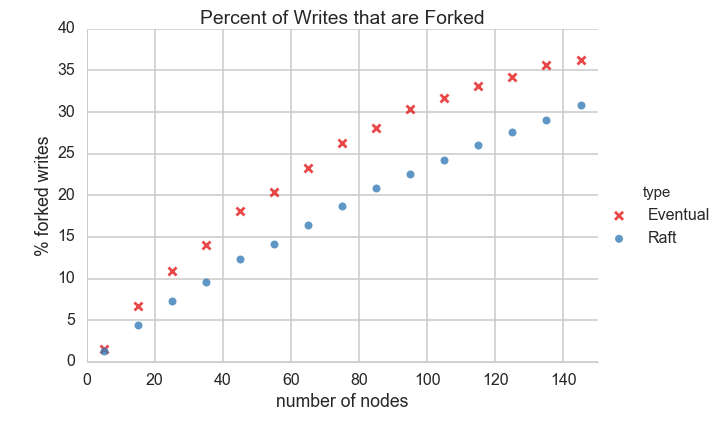
\includegraphics[width=\linewidth]{figures/scaling/forked_writes}
      \caption{Increasing forks in homogenous systems as topology size increases.}
      \label{fig:scaling_forked_writes}
    \endminipage\hfill
    \minipage{0.48\textwidth}
      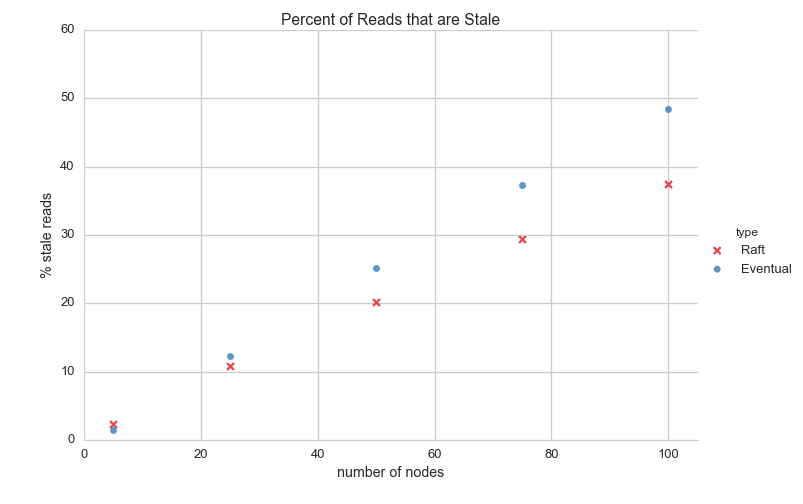
\includegraphics[width=\linewidth]{figures/scaling/stale_reads}
      \caption{Increasing stale reads in homogenous systems as topology size increases.}
      \label{fig:scaling_stale_reads}
    \endminipage
\end{figure*}

\begin{figure*}
    \centering
    \minipage{0.48\textwidth}
      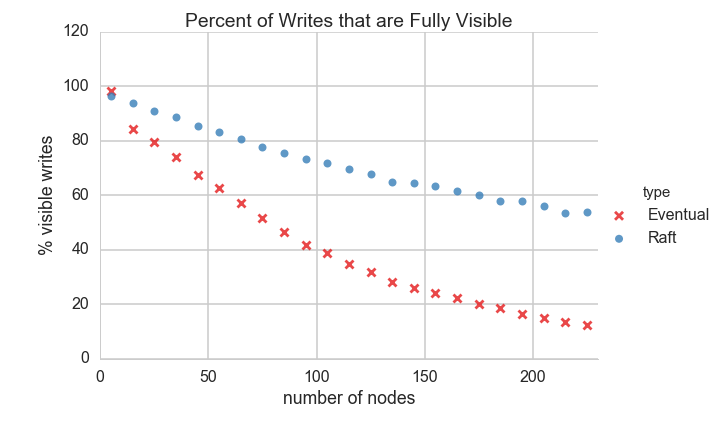
\includegraphics[width=\linewidth]{figures/scaling/visible_writes}
      \caption{Percent of fully visible writes in homogenous eventual and sequential consistency systems.}
      \label{fig:scaling_visible_writes}
    \endminipage\hfill
    \minipage{0.48\textwidth}
      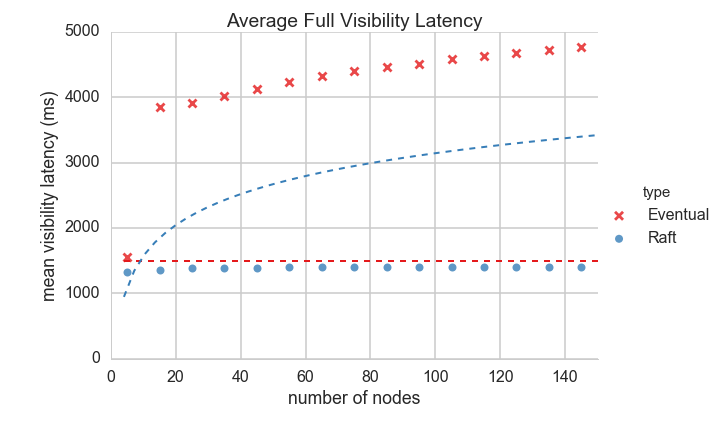
\includegraphics[width=\linewidth]{figures/scaling/visibility_latency}
      \caption{Latency of full visibility in homogenous eventual and sequential consistency systems.}
      \label{fig:scaling_visibility_latency}
    \endminipage
\end{figure*}

As the number of nodes increases, the number of conflicts also increases -- but not the likelihood of a conflict. Our system primarily measures inconsistencies as \textit{forks} and \textit{stale reads}. As shown in Figure \ref{fig:scaling_forked_writes}, the number of conflicts that create forks in Raft is lower than in eventual. This is because eventual consistency relies on fast propagation of updates to minimize forks, which becomes increasingly slow the number of devices in the system, however Raft requires remote writes and voting to commit, introducing a write latency that does not exist in EC. In terms of stale reads, as shown in  Figure \ref{fig:scaling_stale_reads}, there is a cross-over point where anti-entropy initially exceeds the propagation rate of the Raft broadcast interval leading to less staleness, but as the number of nodes increases Raft's broadcast mechanism begins to perform better.

Both of these inconsistencies are directly related to how updates become fully visible in either system. In fact as the number of nodes increases, both systems start to degrade in the percent of writes that become fully visible, though EC far more than raft as shown in Figure \ref{fig:scaling_visible_writes}. For Eventual, this is because the time to visibility is related to the number of pairwise anti-entropy sessions required to propagate a write to all nodes as shown in Figure \ref{fig:scaling_visibility_latency}, where the blue line represents perfect convergence (not likely given uniform random neighbor selection). If an update becomes outdated before it can become fully replicated, it gets ``stomped'', meaning that the later update is propagated over the earlier one. Raft on the other hand only stops writes from becoming fully visible if they are forks, dropping them and rejecting the access to the client who must retry.

We believe that these initial investigations show a critical opportunity: that we can blend the high availability of an eventually consistent system and leverage the best parts of anti-entropy and eventual consistency in network environments where messages cannot get through along with the stability and increased visibility of a strongly consistent core, similar to the central core and flexible outer shell proposed by Gray and Oceanstore \cite{gray_dangers_1996,kubiatowicz_oceanstore:_2000}: we call this \textit{Federated Consistency}. Furthermore, if we can find a way to allocate decision space to a smaller number of nodes, we should be able to scale Raft to greater number of nodes without as steep a curve: we investigate this in \textit{Hierarchical Consensus}. Finally, as suggested by the $T$ timing parameter (though not explicitly covered), the timing measures and performance of consistency protocols are related to the network environment, which is dynamic. Potentially we can improve performance by monitoring the environment and adapting timing parameters to minimize the number of inconsistencies: investigated in \textit{Adaptive Consistency}.

\subsection{Topology}

\begin{figure*}
    \centering
    \minipage{0.5\textwidth}
      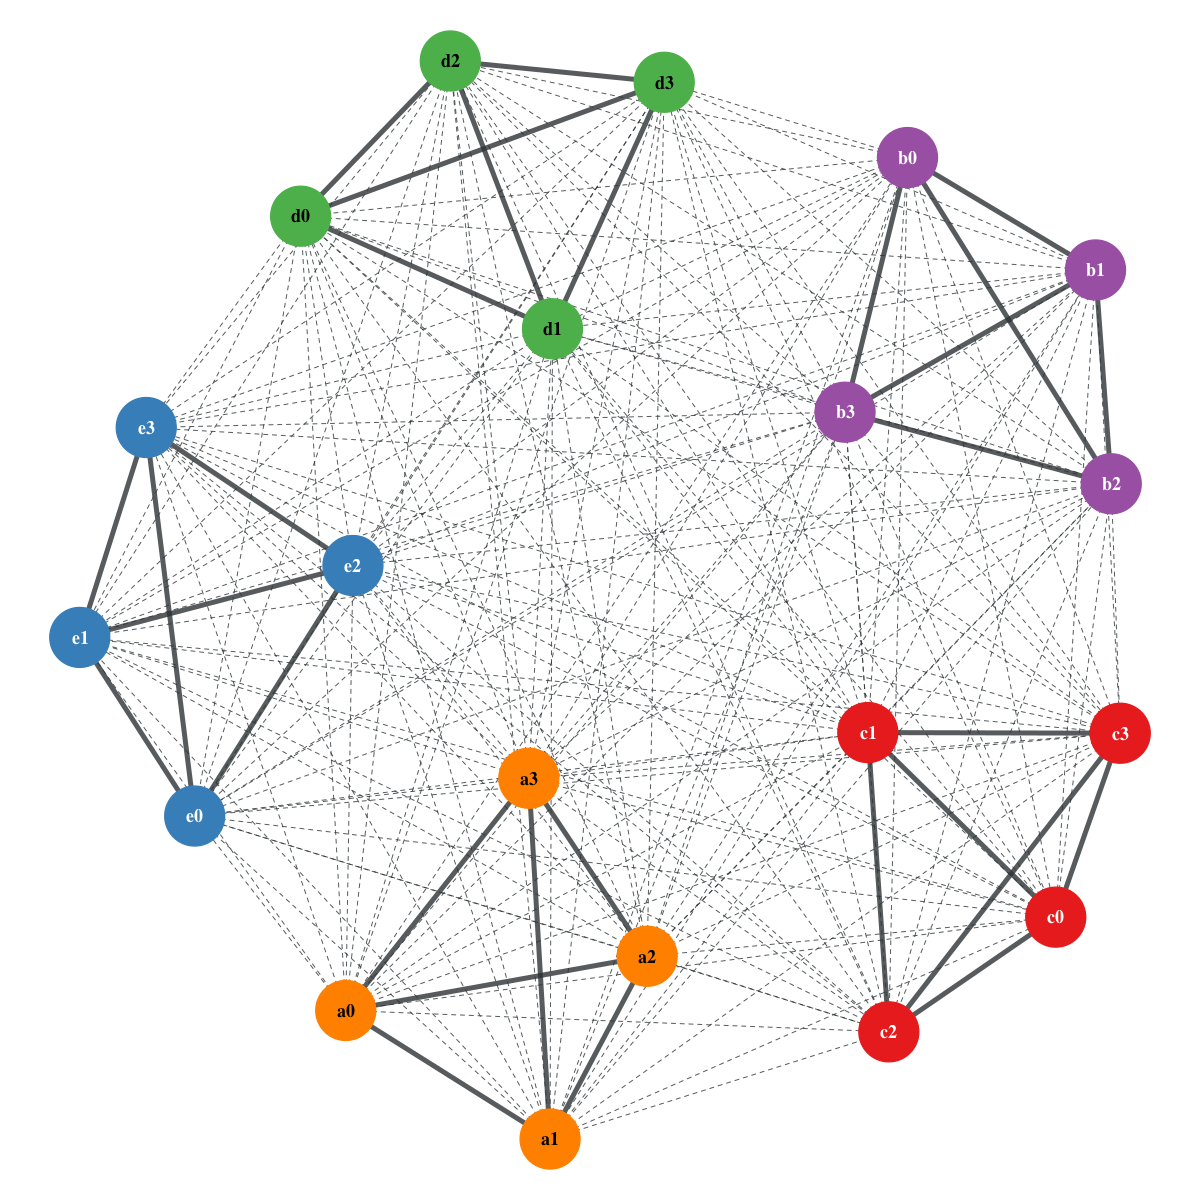
\includegraphics[width=\linewidth]{figures/topology}
      \caption{Proposed Network Topology.}
      \label{fig:topology}
    \endminipage\hfill
    \minipage{0.5\textwidth}
      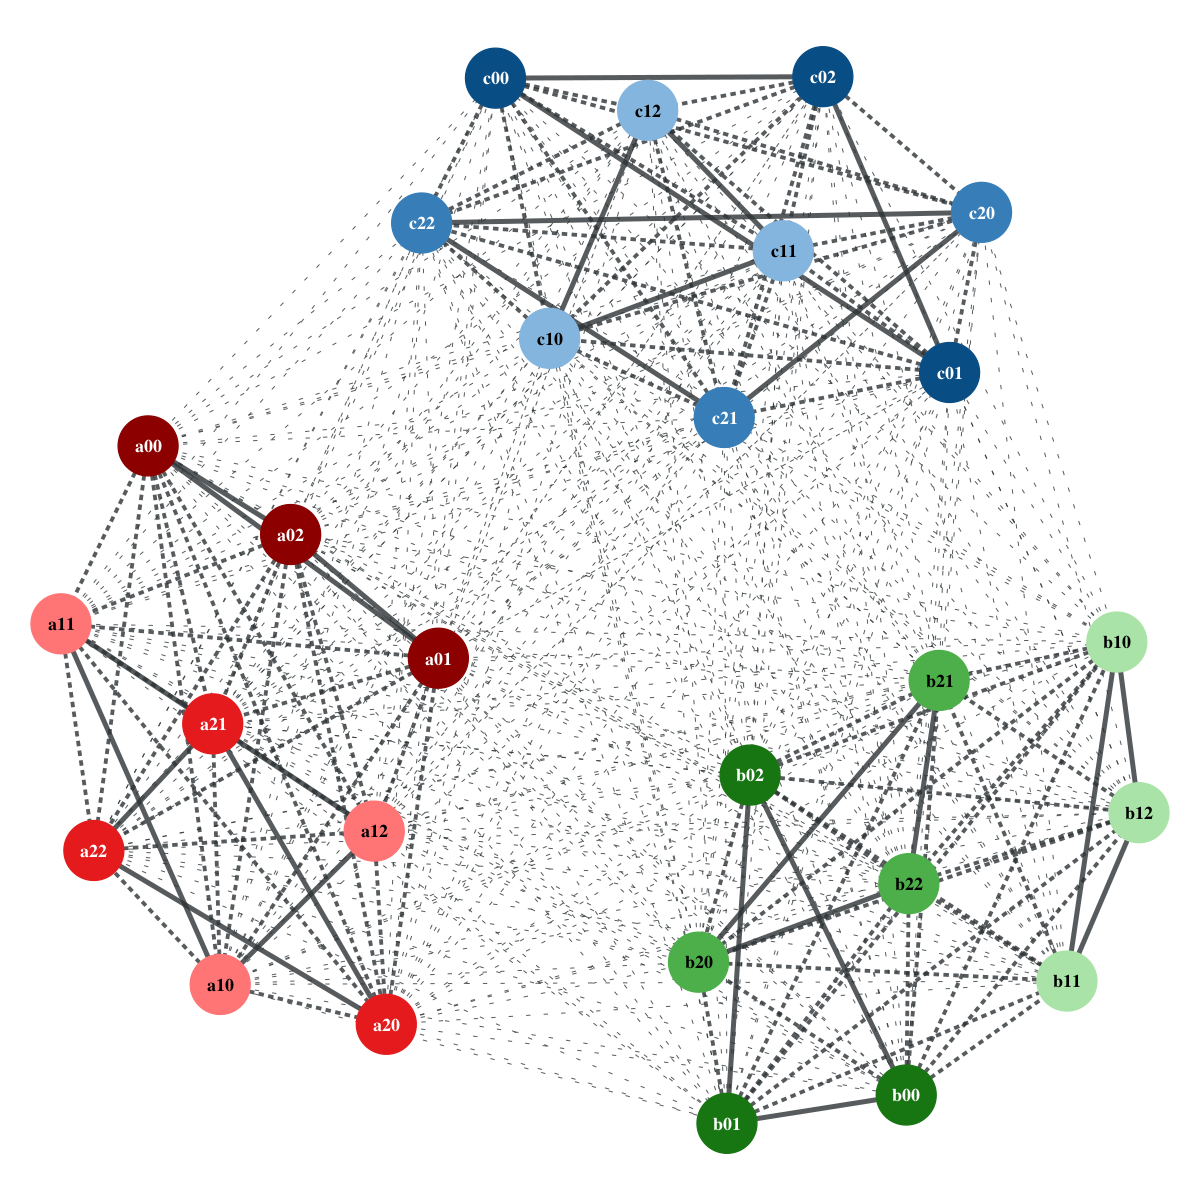
\includegraphics[width=\linewidth]{figures/tiers}
      \caption{Proposed Network Hierarchy.}
      \label{fig:tiers}
    \endminipage
\end{figure*}

As described in the previous section, the primary input to a simulation is the topology of devices and their connections. Topologies allow us to vary connectivity and to simulate a range of network environments, exploring the effect of a variety of consistency protocols in user-centric dynamic clouds. The basic topology discussed in the previous section: multiple locations with variable network connectivity in each location has become a standard model for our research. We propose to investigate a fully connected topology of replica devices each assigned a geographic region as shown in Figure \ref{fig:topology}. Within each region, replica nodes enjoy stable, low-latency connections with their neighbors. However, across regions the latency is higher and the connections variable, meaning that out of order messages and delays are more common across the wide area than in the local area. This topology can be further generalized to tiers of locations as shown in Figure \ref{fig:tiers}, such that groups of nodes are grouped hierarchically in tiers of increasing latency and variability.

Dynamic, user-centric networks are susceptible to routine partitions, events that cause replication messages not to be received. We define two types of communication failure events in our topology: node failure and network partitions. \textit{Node failure} occurs when a single node is shut off or stops responding to messages. \textit{Network partitions} occur when it is not possible for messages to be sent or received from a single geographic region. In both cases, two conditions must be dealt with by the replication protocol in order to satisfy correctness criteria: resending lost messages and bringing nodes that are behind up to date. Introducing these events in our simulation is future work, but is necessary to a complete investigation of consistency in variable network environments.

\subsection{System Description}

Our file system aggregates individual accesses into \textit{Close-To-Open} (CTO) consistency where read and write accesses are ``whole file'' \cite{muthitacharoen_low-bandwidth_2001}. Furthermore, with respect to local accesses we guarantee that a read returns the last write (given no remote updates, \textit{Read Your Writes Consistency}) and that writes are atomic with respect to each other (\textit{Monotonic Write Consistency}) \cite{bermbach_consistency_2013}.

Each replica's log is composed of a series of write accesses to multiple objects. Each object has a unique name that identifies it to the system and a monotonically increasing version number which can be implemented either as a vector clock \cite{parker_detection_1983} (or a simple Lamport scaler) in the case of a fixed topology or as a vector stamp \cite{almeida_version_2002} in the case of dynamic topologies. Therefore a write access encapsulate the following information: the name of the object being written to, the parent version of the object to which the write is being applied, the versions and object names of any other dependencies, the replica id where the write occurred, and an array of blob ids that compose the file at the conclusion of the write.

A read access to a particular object simply looks up the latest local version of that object. Because dependency information can be embedded into a write, it is not necessary to include read accesses in the log. For example, in order to create a transaction that reads from objects $X$ and $Y$, performs a computation then updates objects $Y$ and then $Z$: the write to $Y$ would include as a dependency the earlier version of $Y$ and the read version of $X$ and the write to $Z$ would include the updated version of $Y$ and the read version of $X$. Other notions of dependencies include implicit session dependencies, e.g. all writes are dependent on any access that occur within a minimum time threshold of each other, or explicit dependencies that are added by the application.

Because our system model accounts for heterogenous devices and each write in the log is simply metadata about the version of a file we consider version replication as a separate issue from object or blob replication. Furthermore, system consistency depends only on the replication of version information since a version defines what is visible on each replica to be read (and writes follow an implicit read). While a version must become visible (replicated to) all devices in order for the system to be consistent, the blobs that make up data may not be stored on all devices with different storage resources. If a read access requires blobs that it doesn't have, it can simply request them from a local neighbor that does, or from the origin replica itself.

\section{Proposed Work}

We propose two mechanisms that together will provide responsive, flexible consistency in user-centric dynamic clouds: Federated Consistency and Hierarchical consensus. We hypothesize that the integration of federated consistency models and scalable consensus through these two methodologies will lead to a system that is quantitatively more available (experiences lower aggregate read, write, commit, and visibility latencies) than a homogenous implementation of a sequentially consistent system implemented by Raft. Further we hypothesize that such a system will have stronger consistency guarantees (fewer forks and stale reads) than a homogenous implementation of an eventually consistent file system implemented with bilateral gossip anti-entropy.

Federated Consistency and Hierarchical Consensus provide different opportunities to scale and handle variable environments, each enhancing the other. Federated Consistency allows us to create a flexible, heterogenous distributed system, allowing different replica servers to maintain different consistency levels based on need, but ensuring that global consistency guarantees are met. Hierarchical Consensus extends the Raft consensus protocol to use consensus partitioning as a means of achieving scale and high availability among replicated logs, without sacrificing sequential consistency. We hope to further stretch our proposal to include the investigation of real time optimization and adaptation in response to changing environments. The stretch goal, Adaptive Consistency proposes to utilize both heuristic methods of steering configuration change as well as active, machine learning mechanisms for online optimization.

We propose to confirm our hypotheses in two ways: through the simulation of a variety of network environments and conditions and through real world experimentation on a fully implemented system. The simulation, as discussed in the preliminary work section will allow us to easily explore a variety of environments at a low cost of time and effort. We propose to extend our preliminary work to account for outages and to provide visualizations of consistency protocols. The full implementation will be a distributed file system called \emph{FlowFS} whose architecture is given in Figure \ref{fig:architecture}. By exploring real world workloads in real network environments we will be able to make constructive claims about how consistency needs to evolve as user-centric dynamic clouds become increasingly important.

In this section, we present details of our proposed work. We start with a brief description of Federated Consistency, preliminary work that has already been investigated through use of our simulation. We will then propose a methodology towards hierarchical consensus. Finally, we will propose stretch goals for integrating Federated Consistency and Hierarchical Consensus to become adaptive, automatically responding to changes in the environment. We will conclude with a timeline and goals for paper publications on these topics.

\subsection{Federated Consistency}

Heterogenous topologies with multiple users mean a variety of requirements for both availability and correctness. For example, consider a user working on a non-critical document on a train with limited cellular connectivity; the requirement here is probably high availability and progress rather than strong replication. On the other hand, during collaborative document editing, users might want to ensure strong sequential consistency and are willing to accept minimal delays such that the document is always in a consistent state. However, it is not possible to maintain a single, global consistency level that meets both of these requirements, leading us to the question: can consistency be adapted or tuned at runtime in such a way as to provide more availability in low connectivity situations or for low conflict objects and strong consistency and correctness in optimal network conditions or for critical or high priority workloads?

% Make sure to show that this is work already underway.
Our preliminary solution is a hybridization of discrete consistency models as discussed earlier, which we have already begun exploring via the simulation as introduced in the preliminary work. The Federated Consistency model allows individual replicas to select their own local consistency policies and engage in replication according to the mechanism specified by the policy. Each replica maintains its own local state which is modified in response to local accesses as well as the receipt of messages from remote replicas. Each replica sends messages to other nodes in order to propagate the latest writes as well as to perform housekeeping. Therefore every replica can be seen as an event handler that responds to local access events as well as remote messages and generates more events (sent messages) in return. Simply put, so long as every federated replica has an event handler for all types of RPC messages, federation only has to be defined at the \textit{consistency boundaries}, that is when replicas of one consistency type send messages to that of another.

Given the consistency models discussed in the previous section, we will omit weak consistency as being too simplistic and linearizability as being too performance restrictive. Instead we will focus on the federation of eventual consistency, implemented with latest-writer wins gossip based anti-entropy, and sequential consistency implemented with the Raft consensus algorithm.

A federated consistency protocol finds a middle ground in the trade-off between performance and consistency, particularly between an eventually consistent system implemented via gossip-based anti-entropy \cite{kempe_gossip-based_2003} and a sequential consistency model implemented by the Raft consensus protocol \cite{ongaro_search_2014}. By exploring these two extremes in the consistency spectrum we have observed in simulation that the overall number of inconsistencies in the system is reduced from the homogenous eventual system and that the access latency is decreased from the homogenous sequential system. Moreover, because the global consistency of the system is topology-dependent, it can be said to have flexible or dynamic consistency. We have found that large systems with variable latency in different geographic regions can perform well by allowing most nodes to operate in an optimistic fashion, but maintain a strong central quorum to reduce the amount of global conflict.

\subsubsection{Gossip and Anti-Entropy}

Eventual consistency allows replicas to operate in a highly available fashion at the risk of encountering some conflict (in the form of forks) that must be resolved in the future. We take the common approach of using periodic \textit{anti-entropy} sessions to converge replicas (e.g. reducing entropy, the divergence between the states of individual replicas) via a gossip protocol \cite{kempe_gossip-based_2003}. Each replica periodically selects a random partner and sends a \texttt{Gossip} message containing the latest version of all objects in the replica's local log. On receipt of the \texttt{Gossip} message, the remote replica will compare the RPC object versions with those in its local log. If the RPC versions are later, it will append the later versions of the object to the log (\textit{last-writer wins}). However if the remote object version is later it will send that version back to the originating node in a \texttt{GossipResponse} message. As a result, our anti-entropy implementation is \textit{bilateral}.

Eventual consistency replicas read and write locally, resulting in essentially zero read and write latency. Forks are caused by the \textit{visibility latency}, i.e., the amount of time needed to propagate a write to the rest of the system. The visibility latency is dependent on the number of nodes in the topology and the anti-entropy interval, but because of the bilateral nature of our gossip protocol, has a logarithmic relationship to the number of nodes rather than a linear one.

The relationship between the anti-entropy delay and the size of the network relative to the mean time between accesses potentially means that eventual consistency would not cause forks. Said another way, nothing beats eventual consistency for availability and correctness given a fast enough network. Unfortunately, real-world networks are not ideal and conflicts in an eventual consistent system can lead to behaviors that are especially challenging in file systems. If a partition occurs and an object is forked, both sides of the eventually consistent system will continue allowing the branch to be extended, resulting in a difficult merge. Updates can also be ``stomped'', meaning that if they are not fully replicated they will not continue to be propagated if a later version exists. In order to provide stronger file system semantics, we propose to implement a core strong consistency consensus group that will improve the overall correctness of the system.

\subsubsection{Strong Core Consensus Group}

% \pjk{You've gone from laying out a research plan to describing details of a system. Need to start higher level, and put forward details as ``approaches'' etc.}

We implement sequentially consistent replicated logs via the Raft consensus algorithm~\cite{ongaro_search_2014}. However, consensus alone does not ensure that sequentially consistent file system accesses are guaranteed and a number of policy decisions about how Raft followers read, write and interact with the leader must be discussed. In order to present the possibilities for policies in our system, we must understand the background of the Raft protocol's implementation of sequential consistency.

The Raft leader has the primary responsibility of coordinating all other Raft replicas and therefore is also primarily responsible for ensuring a sequentially consistent system that maintains file system consistency invariants. A write access that originates at a follower must be sent as a \texttt{RemoteWrite} to the leader. The leader accepts writes in the order that they are received, and if the leader detects a fork -- that is that a write has a parent version who already has a child version in the log -- Raft will simply reject (drop) the write. In order to minimize the number of messages that Raft sends, Raft will aggregate all writes into the next \texttt{AppendEntries} message and send them together.

The aggregation of writes and latency of coordination messages means that there is a delay between leadership decisions and follower actions. As a result, write accesses are dependent on the response time of the leader but could also be dropped, requiring the accessor to retry or to handle the conflict somehow. In order to make progress, followers must decide how to read a parent version in order to make a write. There are several options, each providing a varying level of safety, minimizing the risk of a stale read:

\begin{enumerate}
    \item \textit{READ COMMITTED} Raft replicas will only read the latest committed version of an object, guaranteeing that the write will not be rolled back in the case of an outage. However, this read mode introduces the potential for a lot of staleness and therefore forks.
    \item \textit{READ LATEST} Raft replicas will read the latest version of the object in their log, even if it hasn't been committed. Moreover, replicas will read their own local writes rather than waiting for an \texttt{AppendEntries} to return their write.
    \item \textit{REMOTE READ} Rather than read locally, simply request the latest version from the leader. This introduces the potential for additional latency, but may be faster if the expected message latency is less than the heartbeat interval.
\end{enumerate}

Each of these options has critical implications for the likelihood of stale reads and forks in the system. Replicas would choose read committed if the network was highly partition prone and messages from the leader were unstable and prone to being rolled back. Remote read servers replicas well when the average message latency is far lower than the heartbeat interval, though this could be improved by making the heartbeat interval similar to the network latency. For this reason, we propose \textit{read latest} as the most likely scenario for a file system implementing sequential consistency with Raft.

\subsubsection{Integration}

A key requirement of Federated Consistency is the opportunity to create heterogeneous systems with no performance cost, e.g. a homogenous eventual cloud and a homogenous Raft cloud will continue to perform equivalently whether or not they participate in a federated cloud. However, we posit that an eventual cloud should benefit in lowered data staleness and in fork frequency from being connected to a strong, central consensus group. Similarly, Raft nodes should be able to use anti-entropy mechanisms to replicate data and continue writing even if the leader is unavailable and no consensus can be reached to elect a leader. The question is therefore how to integrate the eventual consistency via gossip and sequential consistency via consensus in a non-invasive way.

The central problem is that eventual and Raft clouds choose the ``winner'' of a fork in exactly opposite ways. Eventual clouds choose the last of a set of conflicting writes through a latest-writer wins policy, whereas Raft clouds effectively choose the first by dropping any write that conflicts with any previously seen writes. Our insight is that if the strong central quorum can somehow make an accepted version ``more recent'' than a dropped fork, then the propagation of the fork would cease in the eventual cloud, reducing the possibility of continued forks.

In order to federated multiple consistency models, there are two integration points: communication and consistency. Our initial approach was to integrate communication at the Raft nodes, by allowing Raft nodes to participate in anti-entropy with the eventual cloud (but not other Raft nodes). Eventual nodes therefore ``synchronize'' with a local Raft node (modified by some synchronization probability) by exchanging \texttt{Gossip} messages with the Raft nodes. A slight increase in the synchronization probability balanced the amount of synchronization with the amount of communication in the eventual cloud given the imbalance in the ratio of eventual nodes to Raft nodes. In order to manage the communications delay between the anti-entropy timeout and leadership coordination, Raft nodes must keep local caches of forked or dropped writes so as to not propagate them back to the eventual cloud or replay them to the leader. However, we have observed that this was not enough to stop the eventual cloud from propagating a fork around Raft, causing further inconsistencies.

Our approach to integrate consistency is to extend each version number with an additional monotonically increasing counter called the \textit{forte} (strong) version that can only be incremented by the leader of the Raft quorum. Because the Raft leader dropped forks or any version that was not more recent than the latest version, incrementing the forte number on commit ensures that only consistent versions are marked. In order to determine the latest version, the forte number is compared first, then the version number, allowing Raft to ``bump'' the consistent version to a more recent version. In order to prevent that version's children from becoming less recent, on receipt of a version with a higher forte than the local, eventual nodes must search for the forte entry in their local log, find all children of the update, and set the child version's forte equal to that of the parent.

Our preliminary investigations show that this integration works well to curb inconsistencies due to anti-entropy delays as well as those introduced by communication integration. There are, however, quite a few knobs to turn in the system described above. Further investigation into smoothing integration points between consistency protocols and the policies that each define may lead to smoother messaging with fewer resource constraints. We have identified a current bottleneck in the system however: the leadership of the central quorum, through which every single write must pass, no matter the size of the cloud. In order to address this, we propose an adaptation to the central consensus group such that it can provide Hierarchical Consensus.

\subsection{Hierarchical Consensus}

Federated consistency presents the opportunity to extend distributed storage systems to medium to large scale networks comprised of dozens of replica servers even in the face of high variability in unstable, mobile network environments. By allowing replicas to participate in eventual consistency replication if required to maintain a minimum quality of service, the system becomes flexible enough to handle variability. The key to Federation, however, is the strong central quorum that coordinates partitions in the eventual cloud, handling conflicts and pruning forked branches, minimizing overall inconsistency in the system.

Given the critical nature of the central quorum, a natural question arises: can the quorum scale to meet the availability needs of the Federated system as the topology grows? At a minimum, members of the quorum must be distributed geographically to provide high availability to anti-entropy synchronization requests, requiring at least one quorum node per location. As topologies scale, not only do the number of devices making requests to the leader increase, but so to do the number of objects that must be managed. Finally, as previously shown in Figure \ref{fig:scaling_visible_writes} the number of clients making requests increases, the overall visibility of new versions decreases unacceptably. Larger quorums provide more availability but additional resource requirements.

% Note that Fast Paxos language says "avoid the leader and send directly to acceptors" providing two "paths" to consensus - fast and short. However, I have read other places that this is the equivalent of performing the propose phase in advance of the quorum decision, similar to Raft.
Raft and Paxos optimize the three phase consensus procedure (propose, accept, commit) of quorums by nominating a dedicated proposer, often called the leader or coordinator, who is solely allowed to make voting proposals thus staging the propose phase in advance of any consensus decisions via election. However, the leader is also a single point of failure, and most work in consensus protocols regards correctness and fault tolerance of a system given partitions that remove the leader from connecting to a majority of nodes. Additionally, in order to achieve linearizablity, every single access (including reads) must go through the leader, making the leader a bottleneck whose response performance creates a floor for the overall performance of the system. In order to scale consensus to larger systems, leadership must be addressed.

There are two primary approaches to increasing the availability of the leader in the literature: optimistic ``paths'' and multiple leaders. The former method, implemented in Fast Paxos \cite{lamport_fast_2006}, Egalatarian Paxos \cite{moraru_egalitarian_2012}, and S-Paxos \cite{biely_s-paxos:_2012} allows clients to directly contact acceptors (followers) with proposals, bypassing the leader and distributing leadership activities in a so called optimistic ``fast path''. However, in order to maintain correctness some conflict detection method is required; for example Fast Paxos requires larger quorums for fast path, and Egalitarian Paxos adds dependencies that are checked at ``execution'', where a dependency failure requires a fall back to the ``classic (slow) path''. The latter method allocates the decision space to multiple coordinators either by load balancing multiple quorums as in Multi-Paxos \cite{camargos_multicoordinated_2007} or by utilizing a per-tablet (a grouping of objects) quorum as in BigTable \cite{chang_bigtable:_2008}. Per-tablet quorums also reduce the likelihood of conflicts introducing the possibility of a hybrid approach: optimistic fast paths on multiple quorums with conflict detection and slow path resolution as in MDCC \cite{kraska_mdcc:_2013}.

Unfortunately these approaches, while working well on smaller scale quorum sizes (3-7 nodes), do not scale well in heterogenous and variable-latency environments. Fast-path requires optimism that conflict is relatively rare, otherwise it performs worse than simple classic-path methods since it must implement conflict detection. In larger networks, conflict is more likely, both because of the increased number of writers and owing to message delay. Allocating multiple, small quorums to different decision spaces requires that objects in different tablets be independent of each other; that is, there is no way to order writes sequentially to objects in tablets maintained by separate quorums. Federated consistency, however, requires a single, sequential ordering of all writes to maintain the eventual cloud and many applications of personal clouds that have implicit dependencies not easily embedded as application-level invariants, such as those specified database schemas.

We propose Hierarchical Consensus as a solution to scaling consensus to larger networks while still maintaining a sequential ordering across all objects such that dependencies between objects are determined at runtime. Our approach uses a tiered structure of leadership where the object namespace is governed by a root quorum that partitions the namespace to smaller subquorums via consensus decisions. The set of allocation decisions creates an ordered set of epochs where each epoch defines a specific mapping of objects to subquorums. Accesses on all objects maintained by a single quorum are dependent on each other and \textit{on no other subquorum}. Every access that occurs in a single epoch is said to have \textit{happened before} every access in previous epochs; every write within a subquorum is ordered with respect to that quorum's decisions, and every write between quorums within a single epoch is said to be concurrent.

Hierarchical consensus provides \textit{sequential consistency} on the entire namespace, flexibly allocating consensus decisions to object dependencies which may change over time. Hierarchical consensus is more available due to the use of multiple, smaller quorums and the localization of leadership to where accesses are occurring.

\subsubsection{Consensus Consistency}

In order to implement a sequentially consistent file system with consensus, we must translate the generalized consensus model to a specific consistency model. Generalized consensus protocols do not natively implement any particular consistency and only consider the application of ordered commands to a state machine. Commands generally have no dependencies and agreement considers no invariants beyond whether or not accepting the command would violate global ordering. Therefore to describe the use of a consensus protocol for consistency we must describe approaches such that a consensus decision maintains a consistency invariant. The most obvious is to use consensus to grant locks to replica, object pairs and unlocks once the write has been fully replicated. So long as read/write locks are observed, this system implements linearizeability and is equivalent to two phase commit, though such a system suffers from extremely poor performance.

The approach we take is to make accesses the commands, such that the state machine becomes an ordered series of accesses. If both read and write accesses are applied to the log (meaning that both a read and a write must be remote through the leader) then the system remains linearizable. However, in order to improve performance, we allow reads to occur to the local log of each follower, introducing the possibility of a fork if the local read is behind the global state and a write is submitted that modifies the stale read. Forks are the natural consequence of conflicting accesses and while exacerbated by staleness, are a product of versioning in a file system; local caching only makes the problem slightly worse. In order to maintain the no-forks invariant, leaders must therefore check writes to detect forks and drop those that are.

\begin{figure}
    \centering
        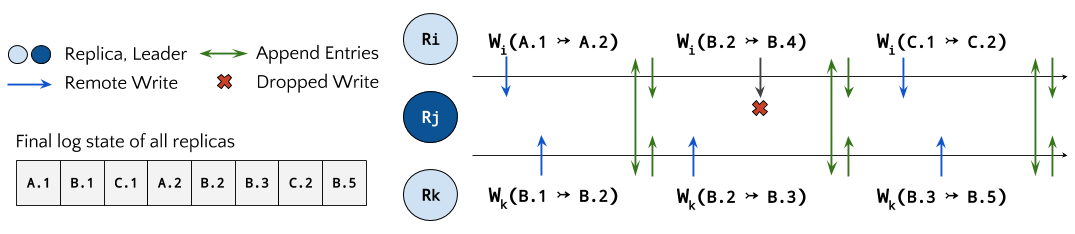
\includegraphics[width=.9\textwidth]{figures/ordered}
        \caption{Sequential ordering in consensus based file system}
        \label{fig:ordered}
\end{figure}

Consider the simple example shown in Figure \ref{fig:ordered}, implemented using the Raft protocol where writes are aggregated in \texttt{AppendEntries} (shown as green lines that occur routinely every heartbeat interval). In this example the object namespace is the set $\{A, B, C\}$ and each version is represented as the object name dot annotated with a monotonically increasing version number (we presume that version 1 of each object has already been written to the log). A write is conducted by reading the latest version of the object and writing the new version, therefore a write by replica $i$ that reads version $n$ and writes to version $m$ on object $O$ is given as follows: $W_i(O.n \rightarrowtail O.m)$.   Writes are ordered with respect to their arrival at the leader ($R_j$), are appended to the logs of the followers on \texttt{AppendEntries}, are committed by the leader when a majority of followers responds affirmative to the append RPC, and are marked as committed by followers on the subsequent \texttt{AppendEntries}. The leader must reject $W_i(B.2 \rightarrowtail B.4)$ in order to maintain consistency because that write would cause a fork to occur in the log. The final log is identically ordered on all replicas for all objects, therefore we can say we have achieved sequential consistency such that every write that appears in log position $i$ happens before ($\rightarrow$) the log entry at $i-1$.

In this example, we have only nominated one \textit{explicit} dependency on each write, the parent version, and enforced a no-forks invariant as a policy on this dependency at the leader. A consequence of this style consistency is the \textit{implicit} causality of all prior writes to a given write. For example, $W_i(C.1 \rightarrowtail C.2)$ implies implicit dependencies on $A.2$ and $B.3$, e.g. any versions that could have possibly been read prior to the write (and also the reason that reads must be logged in order to achieve linearizability). Similarly $W_k(B.3 \rightarrowtail B.5)$ has implicit dependencies on $A.2$ and $C.1$, more closely inspecting the log we can see that $C.2 \rightarrow B.5$ and $C.1 \rightarrow C.2$ therefore by transitivity, $C.1 \rightarrow B.5$, a correct interpretation of the log and implicit dependencies.

While implicit dependencies are critical to consistency, we observe that it is unlikely that a write is truly dependent on every historical write but is rather dependent on a local, recent subset of the namespace \cite{bailis_potential_2012}. Hierarchical consensus therefore makes use of \textit{explicit} causality to allocate the namespace to subquorums in order to balance the leader workload. This has several implications including allowing the ability to lock the ownership of a series of critical files, to specify particular replicas as stable storage for high value data, or to maintain policies and invariants that go beyond ordering; for example spatial polices (what data gets stored), temporal policies (what versions are stored) and synchronization policies (how and when replication occurs).

\subsubsection{Namespace Allocation}

\begin{figure}
    \centering
        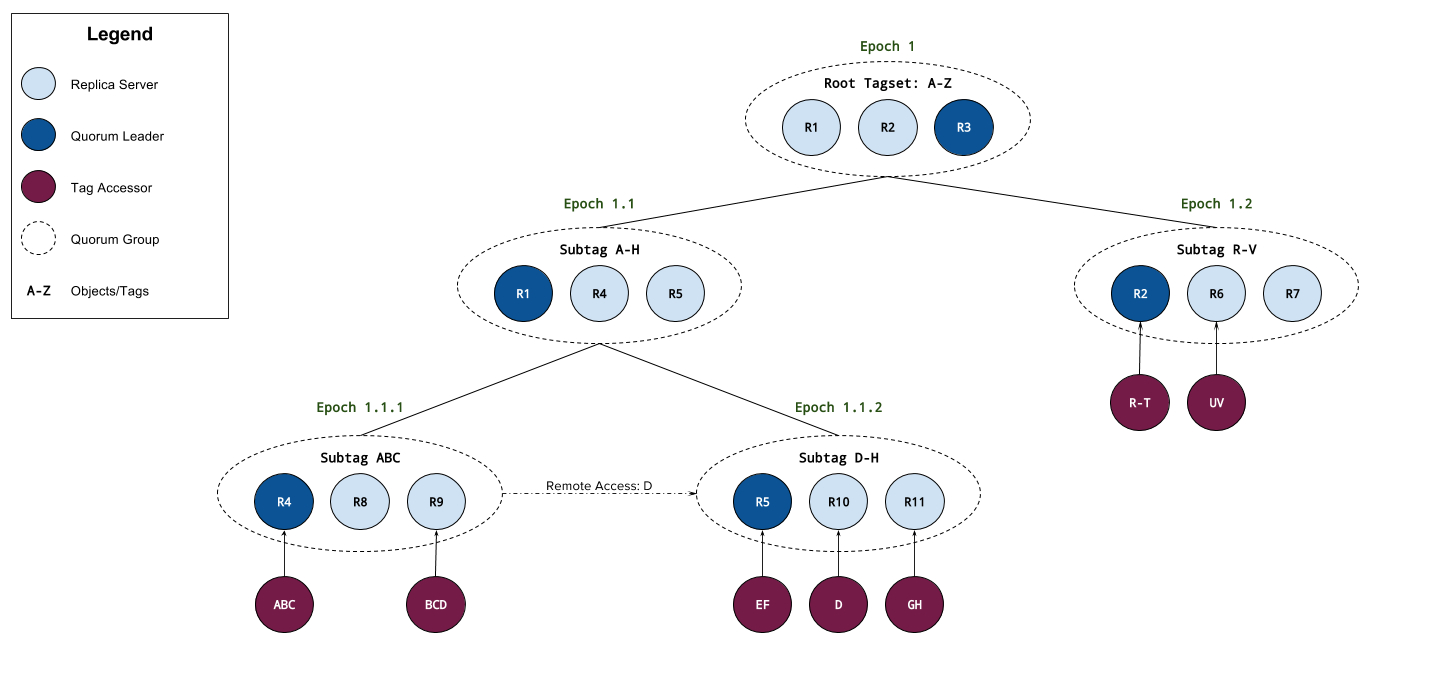
\includegraphics[width=.9\textwidth]{figures/hierarchical}
        \caption{Hierarchical consensus partitions the namespace across subquorums}
        \label{fig:hierarchical}
\end{figure}

An open question for our research is how to automatically allocate the namespace such that leadership of a subset of the namespace is local to the accesses and that members of the quorum are distributed to provide wide area durability and availability. The goal of allocation, is shown in Figure \ref{fig:hierarchical} - a hierarchy of quorums such that the children of each tier manage consensus decisions on a non-overlapping portion of the namespace.

Consider a motivating example using the notion of \textit{sessions}. Starting from a quiescent state (no accesses), a node or a group of nodes begins reading and writing to a set of objects (perhaps collaborative editing of a document, or a series of financial transactions); we expect that after some finite amount of time, the access pattern will change or cease. We can therefore state that all objects involved in a single session are explicitly causally related to each other and to no other objects in the namespace. Whether we describe sessions as a fixed, sliding window or as something more variable, some automatic determination that those objects should be coordinated together is necessary. To that end we will define a \textit{tag} as a time-annotated subset of the namespace and a \textit{tagspace} as the set of non-overlapping tags that compose the namespace for a given time period.

Hierarchical consensus starts with a root quorum whose responsibility is to govern the entire namespace. The root quorum does so by maintaining a root \textit{epoch}, a monotonically increasing counter which identifies the current \textit{tagspace}. In addition to consensus decisions related to leader election, accesses, and membership changes, decisions that modify the tagspace also require consensus. We define two primary operations: \textit{split} creates a new subquorum, splitting a larger tag from the previous tagspace and \textit{join} removes a subquorum, joining two smaller tags from the previous tagspace. Any decision that modifies the tagspace (thus creating a new tagspace) requires an increment of the \textit{epoch}.

The fundamental relationship between accesses in epochs is as follows: any access that happens in epoch $i$ happened before every access in epoch $i-1$; accesses in different tags but in the same epoch happen concurrently from the global perspective, but are ordered locally in the quorum that governs that tag. As a result, every log has a determined, sequentially consistent and correct ordering, though the logs of two individual replicas may differ. Hierarchical consensus cannot provide linearizability, but does provide sequential consistency.

\subsubsection{Operation}

\begin{figure}
    \centering
        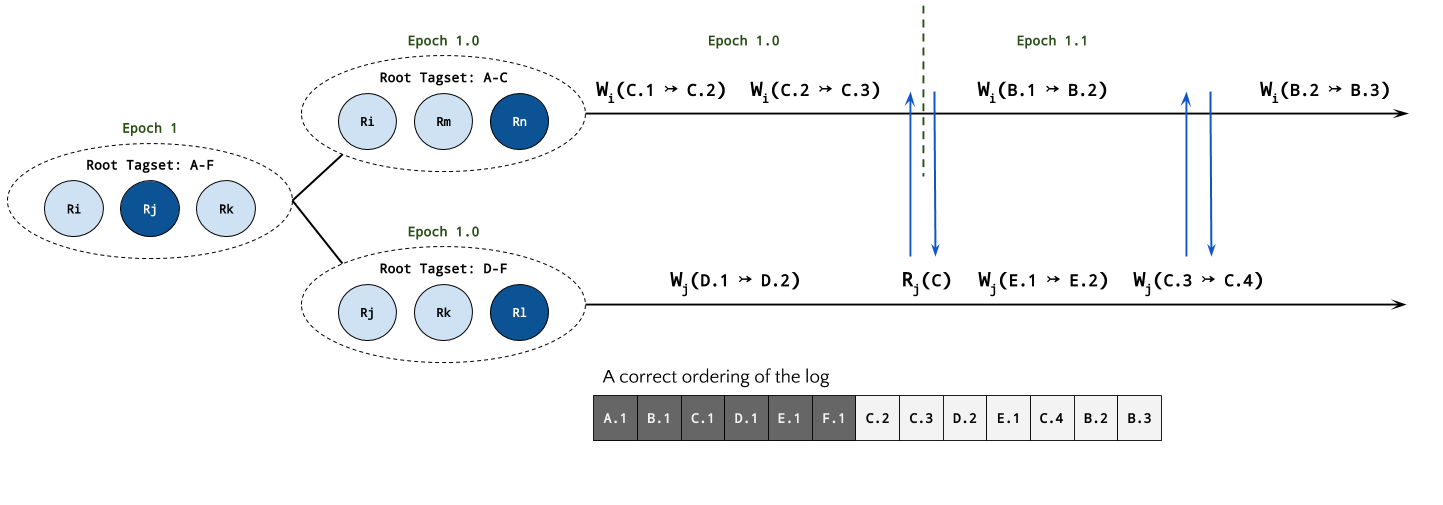
\includegraphics[width=.9\textwidth]{figures/subepoch}
        \caption{Sub-epochs allow remote accesses between tags without a tagspace change.}
        \label{fig:subepoch}
\end{figure}

The namespace allocation creates a tiered structure of leadership such that the root quorum is responsible for the entire namespace, subquorums are responsible for tags, and leaves are responsible for handling accesses to their tag. Any access to an object must be forwarded as a remote access to the leader of the quorum that handles the tag that encapsulates the object. The only exception is the optimization made for members of the quorum who can read locally any object in their tag space. By optimizing the locality of access and spreading the workload to multiple leaders, we hope to show that the overall performance of the system increases.

When a member of a quorum wishes to access an object that is not in that quorum's tag, one of two things must happen: either a tag decision must be made to reallocate the tag space such that it is local to the new accessor or some mechanism must allow remote accesses between quorums. The former case is expensive, but if the accesses to that object become routine then the upfront cost will pay for future accesses. However, for non-routine accesses some mechanism for remote access is required.

The issue is that a remote access from one tag to another creates an implicit dependency between all accesses that happened before the remote access and all those that follow the local one. Correctness is maintained by the ordering of epochs, so some local split is required. Consider the example in Figure \ref{fig:subepoch}: the remote read access, $R_j(C)$ implies any writes to tag $D-F$ following the read depends an all writes in tag $A-C$ that occurred before the read. Furthermore, the remote write $W_j(C.3 \rightarrowtail C.4)$ is a non-conflicting write, depends on all writes on tag $D-F$ that happened before \textit{and} depends on all writes in tag $A-C$ that occurred before the remote read, and occurs concurrently with any writes that happen after so long as there is no conflict.

Our proposed solution is similar to the epoch solution: each tag quorum maintains a per-epoch, monotonically increasing sub-epoch counter. In the case of a remote access, that counter is incremented to demarcate the ordering of all accesses in the tag that happened before the remote access and all those that follow. This counter must be replicated in addition to the version number, and can therefore be seen as an explicit dependency applied to all remote writes. As a result, any quorum that receives these ordering indicators can appropriately order their logs.

This mechanism also leads us to suspect that generalizing the consensus hierarchy to arbitrarily deep levels is possible; particularly since the notion of sub-epoch numbers already exists. Clearly some coordination is required to ensure that tag space changes filter down to all leaf nodes, and that is the primary subject of our future work related to this proposal.

In addition to correctness, we also propose to show failure tolerance by utilize Raft-style quorum mechanics. There are two distinct kinds of failure in a hierarchical system: replica failures (a single node crashes and dies) and partitions, where parts of the network are cut off from receiving messages. We believe that we can model failure tolerance from both of these perspectives through a formulation of quorum size, minimal intersection set between quorums, and the depth/breadth of the hierarchy. We propose to show correctness in the face of failure in the least and will stretch to show inherent robustness due to the structure of the hierarchy.

\subsection{Adaptive Consistency}

Federated Consistency attempts to provide heterogenous devices in a user-centric dynamic cloud the ability to set their consistency level as needed. We propose to show that a small, strong central quorum can improve the global consistency of the system while allowing for local availability. Hierarchical consensus expands the strong central quorum, providing high throughput on the leader of the quorum by allocating multiple leaders for different objects. Together, Federated Consistency and Hierarchical Consensus provide mechanisms that deal with unstable network environments and the unique challenges a multi-user, multi-device system may encounter. However, neither Federated nor Hierarchical deal with the dynamic or mobile nature of the network; and while they provide responsiveness at the user layer, cannot take advantage of boosts in bandwidth or respond to gaps our outages.

Therefore we propose the final step in the study of user-centric dynamic clouds is the real time adaptation of the network according to observed latency values. We have observed that eventually consistent nodes can change their timing parameters at will to take advantage of lower latencies or to save work in sparse network conditions. While joint consensus may be required to adapt the parameters of a consensus group, lowering the timing parameter dramatically improves throughput and commit latency and in the face of increasing latency, ensuring that the timing parameters are conservative enough such that messages aren't received out of order or such that ``leader thrashing'' occurs as much delayed heartbeat messages cause candidacies.

By equipping the system with online monitoring of local network conditions and access patterns, we propose to investigate heuristics and optimizations that can improve performance. In particular, these heuristics can be used to provide a history of performance to the user and recommendations of how to changing timing parameters, topology, or consistency model to adapt. Heuristics can also be used to adapt the policies of different machines in different networks; for example a laptop could participate in hierarchical quorum while at the office or at home, but allow eventual replication while mobile.

Finally, we believe that by constant observing of accesses patterns and the network, we can use machine learning techniques to classify access patterns, detect potential conflicts or anomalies in the network or environment, or to cluster similarly accessed objects to ensure they were always in the same tag. These techniques would automatically and actively adapt the federated system, improving performance in real time and relearning through online techniques and reinforcement from user behavior.

\section{Timeline}

In order to meet the requirements of this proposal and provide substantive results for a dissertation, we propose to undertake the following projects, along with their given priority and timeline.

\begin{center}
\begin{tabular}{|l c|c|}
\hline
Project & Priority & Time Estimate \\
\hline
Simulation of Federated Consistency & $\bigtriangleup$ & 1 months \\
Simulation of Hierarchical Consensus & $\bigtriangleup$ & 2 months \\
Implementation of the FlowFS & $\bigtriangleup$ & 3-4 months \\
Evaluation of FlowFS on real workloads & $\bigtriangleup$ & 2-3 months \\
Proof of correctness and consistency & $\bigtriangleup$ & 1 month \\
Heuristics to optimize and allocate FlowFS & $\bigtriangledown$ & 1 month \\
Online optimization and consistency adaptation & $\bigtriangledown$ & 2-3 months \\
\hline
\multicolumn{2}{|l|}{\textbf{TOTAL}} & 12-16 months \\
\hline
\end{tabular}
\end{center}

After investigations and evaluations of Federated Consistency and Hierarchical Consensus in simulation, I propose to implement a file system utilizing both mechanisms and verify the system meets consistency requirements on large networks in real world workflows. Goals marked with $\bigtriangleup$ indicate necessary checkpoints to the successful completion of the dissertation, including some proof of correctness. I further propose the stretch goals (marked with $\bigtriangledown$) of real time adaptation and online optimization, investigating the application of both heuristics and active machine learning techniques to learn usage patterns and improve consistency and performance.

Based on preliminary work done in simulation as well as the above timeline, I propose the following paper and conference submission goals:

\begin{center}
\begin{tabular}{|l|l|l|c|c|}
\hline
Paper & Title & Location & RFP & Date \\
\hline
Federated Consistency & IEEE ICDCS 2017 & Atlanta, GA & Dec 5, 2016 & Jun 5-8 2017 \\
% http://icdcs2017.gatech.edu/
% IEEE International Conference on Distributed Computing Systems

User-Centric Dynamic Clouds & ACM HotStorage 2017 & Santa Clara, CA & N/A & Jul 10-11, 2017 \\
% https://www.usenix.org/conferences
% ACM Hot Topics in Storage and File Systems 2017

Hierarchical Consensus & ACM PODC 2017 & Washington DC & Feb 10, 2017 & July 2017 \\
% http://www.podc.org/
% ACM Principles of Distributed Computing

Hierarchical FlowFS & ACM SOSP 2017 & Shanghai, China & Apr 21, 2017 & Oct 29-31, 2017 \\
% https://www.sigops.org/sosp/sosp17/index.html
% ACM Symposium on Operating Systems Principles

Responsive Consistency & USENIX NSDI 2018 & N/A & N/A & N/A \\
% https://www.usenix.org/conference/nsdi17
% USENIX Symposium on Networked Systems Design and Implementation

\hline
\end{tabular}
\end{center}

\section{Conclusion}

In this proposal we have presented two novel approaches to provide responsiveness in user-centric dynamic clouds: Federated Consistency and Hierarchical Consensus, as well as stretch proposals related to automatic Adaptive Consistency. Research into these approaches is important because the number of computing devices per person is increasing and new devices are coming online via the Internet of Things. Current approaches of centralized, cloud distributed data storage provide mobile availability and durability, but do not lend themselves well to multi-user, collaborative environments. We believe that as a result, user-centric dynamic personal clouds will become increasingly important to support the increase in the number of local devices.

We have grounded our proposal in consistency, consensus, and replication. A generalized consistency model shows that consistency is a scale along dimensions of ordering and staleness; we have extended this model to account for file-system specific semantics and specifically measure forks and stale reads, symptoms of inconsistent ordering. Consensus allows the strong coordination of a distributed system, and we specifically consider the Raft consensus protocol. Finally, replication via anti-entropy gossip and broadcast protocols must consider resource constraints. By applying consistency only to the metadata of objects and by replicating immutable data blocks, we believe that a global, scalable network file system is possible.

We propose to show through simulation and through a file system implementation that Federated Consistency and Hierarchical Consensus together will lead to a highly available system with strong consistency guarantees. Federation will make use of a strong-central quorum to synchronize an eventual cloud, minimizing overall inconsistency in the system, while allowing eventual nodes to make progress with reduced coordination requirements. The central quorum needs to be able to scale to dozens or hundreds of nodes and so we propose Hierarchical Consensus as a means of partitioning consensus decisions to particular objects across the namespace to different leaders. This load balancing will increase throughput but also increase correctness. Together and with potential future research into online optimization we believe that this research will lead to a high quality dissertation.

\newpage

\appendix
\section{Reading List}
\label{app:readinglist}

\subsection{Consistency}

1) \bibentry{lamport_time_1978}

2) \bibentry{bermbach_consistency_2013}

3) \bibentry{terry_managing_1995}

4) \bibentry{bailis_quantifying_2014}

5) \bibentry{lloyd_dont_2011}

6) \bibentry{bailis_potential_2012}

7) \bibentry{almeida_version_2002}

8) \bibentry{attiya_sequential_1994}

9) \bibentry{liu_warranties_2014}

10) \bibentry{corbett_spanner:_2013}

\subsection{Consensus}

1) \bibentry{thomas_majority_1979}

2) \bibentry{lamport_paxos_2001}

3) \bibentry{chandra_paxos_2007}

4) \bibentry{lamport_fast_2006}

5) \bibentry{camargos_multicoordinated_2007}

6) \bibentry{ongaro_search_2014}

7) \bibentry{howard_raft_2015}

8) \bibentry{lampson_how_1996}

9) \bibentry{li_hierarchical_2014}

10) \bibentry{zhang_hierarchical_2007}

\subsection{Replication}

1) \bibentry{stoica_chord:_2001}

2) \bibentry{kubiatowicz_oceanstore:_2000}

3) \bibentry{gray_dangers_1996}

4) \bibentry{venkataramani_operating_2002}

5) \bibentry{kraska_mdcc:_2013}

6) \bibentry{mashtizadeh_replication_2013}

7) \bibentry{karp_randomized_2000}

8) \bibentry{kempe_gossip-based_2003}

9) \bibentry{li_secure_2004}

10) \bibentry{keleher1999decentralized}

\newpage
\section{FlowFS Architecture}
\label{app:architecture}

\begin{figure}[h!]
    \centering
        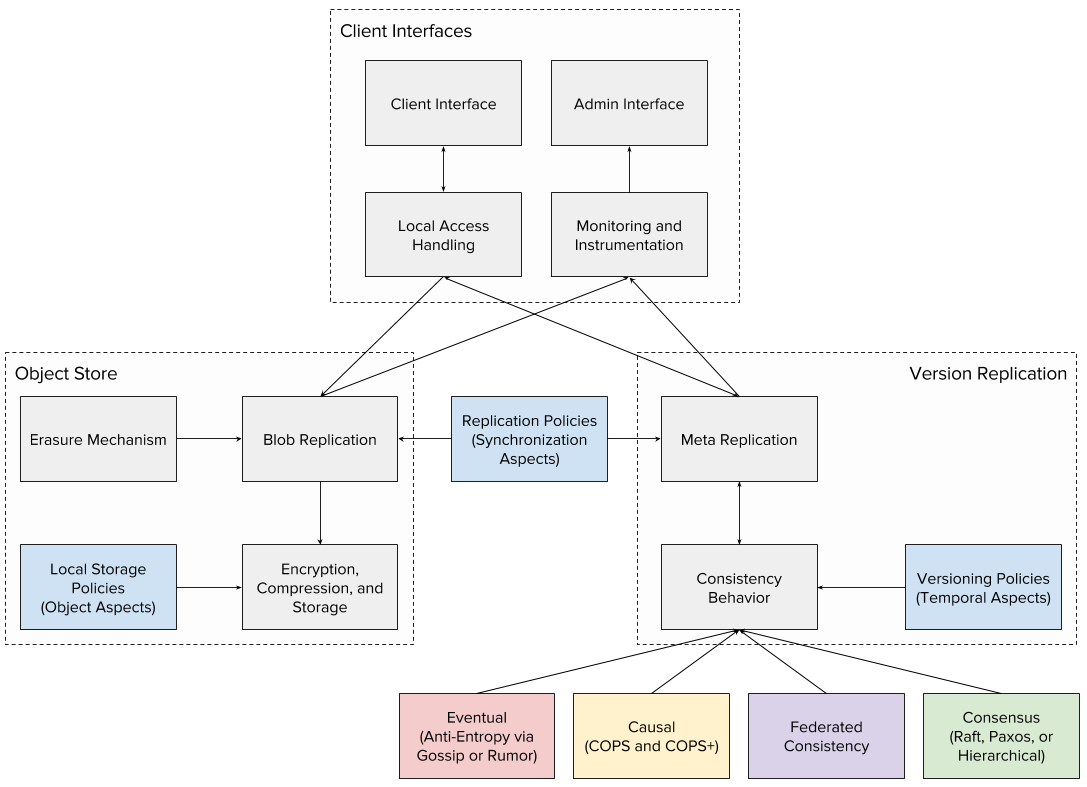
\includegraphics[width=\textwidth]{figures/architecture}
        \caption{Component architecture of FlowFS, our proposed file system.}
        \label{fig:architecture}
\end{figure}

% \newpage

% \section{Appendix B}
% \label{app:cvtdp2r}


\newpage

\bibliographystyle{plain}
\bibliography{prelim}

\end{document}
